\documentclass[12pt, a4paper]{article}

\usepackage[utf8]{inputenc}

% Limit the page margin to only 1 inch.
\usepackage[margin=1in]{geometry}

%Imports biblatex package
\usepackage[
backend=biber,
style=alphabetic
]{biblatex}
\addbibresource{../math-342w.bib}

% Enables the `align' environment.
\usepackage{amsmath}
\usepackage{bm}

% Provides useful environments, such as:
% - \begin{proof} ...\end{proof}
\usepackage{amsthm}
\newtheorem{proposition}{Proposition}
\theoremstyle{definition}
\newtheorem*{definition}{Definition}
\newtheorem{theorem}{Theorem}
\newtheorem{corollary}{Corollary}

% Enables using \mathbb{}, for example \mathbb{N} for the set of natural numbers.
\usepackage{amssymb}

% Allows using letters in enumerate list environment. Use, for example:
%\begin{enumerate}[label=(\alph*)]
% ...
%\end{enumerate}
\usepackage[inline]{enumitem}

% Enable importing external graphic files and provides useful commands, like \graphicspath{}
\usepackage{graphicx}
% Images are located in a directory called "images" in the current directory.
\graphicspath{{./images/}}

% Make links look better by default.
% See: https://tex.stackexchange.com/questions/823/remove-ugly-borders-around-clickable-cross-references-and-hyperlinks
\usepackage[hidelinks]{hyperref}
\usepackage{xcolor}
\hypersetup{
	colorlinks,
	linkcolor={red!50!black},
	citecolor={blue!50!black},
	urlcolor={blue!80!black}
}

% Code Listings. Source:
% https://stackoverflow.com/questions/3175105/inserting-code-in-this-latex-document-with-indentation
\usepackage{listings}
\usepackage{color}
\usepackage[most]{tcolorbox}

\definecolor{dkgreen}{rgb}{0,0.6,0}
\definecolor{gray}{rgb}{0.5,0.5,0.5}
\definecolor{mauve}{rgb}{0.58,0,0.82}

\lstset{frame=tb,
	language=Java,
	aboveskip=3mm,
	belowskip=3mm,
	showstringspaces=false,
	columns=flexible,
	basicstyle={\small\ttfamily},
	numbers=none,
	numberstyle=\tiny\color{gray},
	keywordstyle=\color{blue},
	commentstyle=\color{dkgreen},
	stringstyle=\color{mauve},
	breaklines=true,
	breakatwhitespace=true,
	tabsize=3
}

\newcommand{\prob}{\text{P}}
%\newcommand{\complement}{\mathsf{c}}
\title{Lecture 12: MATH 342W: Introduction to Data Science and Machine Learning}
\author{Sergio E. Garcia Tapia\thanks{Based on lectures of Dr. Adam Kapelner at Queens College.
See also the \href{https://github.com/kapelner/QC_MATH_342W_Spring_2025}{course GitHub page}.}}
\date{March 18, 2025 (last updated \today)}

\begin{document}
	\maketitle
	\section*{Overfitting}
	Recall the three types of error we discussed in lecture 3:
	\begin{itemize}
		\item \textbf{Ignorance error}: This is given by $t-f=\delta$, where $t$ is the ``true"
		function for the phenomenon with true driver inputs $z_1,z_2,\ldots,z_t$,
		and $f$ is the ``best" function that takes our predictors $x_1,x_2,\ldots,x_p$
		and uses them as proxies to the true drivers. 
		\item \textbf{Misspecification Error}: Given by $f-h^*=\epsilon-\delta$, it occurs
		from choosing a candidate set of functions that do not necessarily capture
		the function form of $f$.
		\item \textbf{Estimation Error}: Given by $h^*-g$, incurred by the fact that
		even though $h^*$ is the best function from our candidate set, an algorithm
		$\mathcal{A}$ produces $g$ and cannot hope to produce $h^*$.
	\end{itemize}
	What type of error results from overfitting? It's not ignorance error because
	the number of real features is not changing; by adding junk features the amount
	of information does not change, we do not know anything more, and also not
	anything less. It's also not misspecification, because even though we discussed
	our theory in the context of OLS, the same ideas applies to other models, such
	as logistic regression, and overfitting can occur there.
	
	That leaves estimation error. Suppose the \textit{true model} is
	\begin{align*}
		h^*(\mathbf{x}) = \beta_0 + \beta_1 x_1 + \cdots + \beta_1 x_p
	\end{align*}
	Now suppose we add a \textit{fake} predictor:
	\begin{align*}
		h^*(\mathbf{x})
		= \beta_0 + \beta_1 x + \cdots + \beta_p x_p + {\color{red} \beta_{fake} x_{fake}}
	\end{align*}
	Then $\beta_{fake}=0$ since predictor $x_{fake}$ has nothing to do with
	our phenomenon. However, our algorithm $\mathcal{A}$ will output:
	\begin{align*}
		g(\mathbf{x}) = b_0 + b_1 x_1 + \cdots + b_p x_p + {\color{red}  b_{fake} x_{fake}}
	\end{align*}
	Since we are projection the response vector $\mathbf{y}$ onto a new dimension,
	in the direction of $\mathbf{x}_{fake}$, the projection of $\mathbf{y}$ is unlikely to
	be zero, and hence $b_{fake}\neq 0$ (see Figure~\ref{fig:project-xfake}).
	\begin{figure}
		\centering
		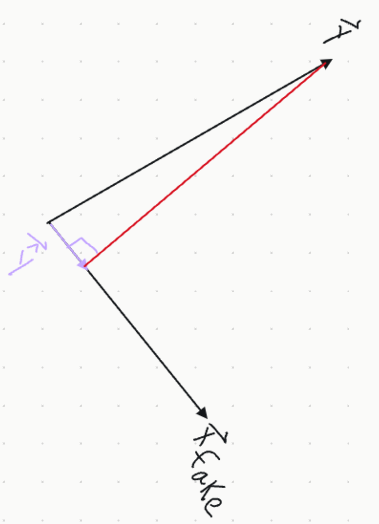
\includegraphics[width=0.25\textwidth]{project-onto-fake-feature}
		\caption{Projecting $\mathbf{y}$ in the direction of some vector $\mathbf{x}_{fake}$
		that accounts for feature $x_fake$.}
		\label{fig:project-xfake}
	\end{figure}
	The $b_fake$ will cause more estimation error ($h^*-g$). To measure estimation error,
	in theory we can use $\|\bm{\beta}-\mathbf{b}\|^2$, which approaches $0$ as
	$n\to\infty$ (holding $p$ constant; this is proved in MATH 343). In the real
	world, however, we don't know $\bm{\beta}$.
	\section*{Honest Performance Metrics}
	What can we do to obtain honest performance metrics? As we saw, in-sample is dishonest
	because it cannot be \textit{detect} when we add projections onto garbage features.
	Using our current approach, $b_{fake}$ will cause our model to yield errors in the future.
	
	Instead, we can calculate performance on future data, as depicted in Figure~\ref{fig:future-data}
	\begin{figure}
		\centering
		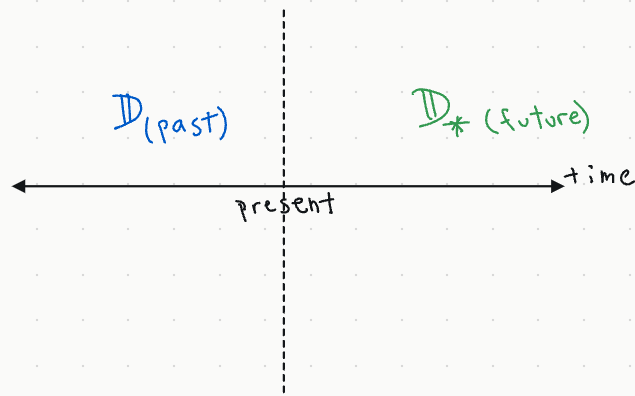
\includegraphics[width=0.3\textwidth]{future-data}
		\caption{Using future data $\mathbb{D}_*$ to test performance of model
		built using $\mathbb{D}$.}
		\label{fig:future-data}
	\end{figure}
	The metrics computed on $\mathbb{D}_*$ are called \textbf{out-of-sample (oos)}
	because they do not come from the data set we used to build $g$.
	Let $n_*$ be the number of units in $\mathbb{D}_*$. Let $e_{*1},\ldots,e_{*n_*}$
	be the OLS residuals, where
	\begin{align*}
		e_{*i}:=y_{*i}-\hat{y}_{*i}\\
		\hat{y}_{*i} := g(\mathbf{x}_{*i})
	\end{align*}
	Then we can define
	\begin{align*}
		oosSSE &:= \sum_{i=1}^{n}e_{*i}^2\\
		oosMSE &:= \frac{oosSSE}{n_*}\\
		oosRMSE &:= \sqrt{oosMSE}\\
		oosSST &:= \sum_{i=1}^{n_*}(y_{*i}-\bar{y}_*)^2\\
		oosR^2 &:= 1 - \frac{oosSSE}{SST_*}
	\end{align*}
	Note that for the $oosMSE$, we no longer need the insurance 
	of subtracting $p+1$ in the denominator. Also, $oosR^2\leq 1$, but it can be
	negative; the result we proved for OLS does not hold here. $oosR^2$ is negative,
	then our model performs poorly.
	\section*{Using Future Data}
	The problem we now face is that, in general, we do not have data $\mathbb{D}_*$
	with future data. What do we do in this case? We partition the data we already have!
	\begin{align*}
		\mathbb{D} &= \mathbb{D}_{\text{train}} \cup \mathbb{D}_{\text{test}}\\
		\varnothing &= \mathbb{D}_{\text{train}} \cap \mathbb{D}_{\text{test}}
	\end{align*}
	Specifically, we split along rows, where each row is a separate observation.
	Let $\mathbb{D}_{\text{train}}$ be the historical data used to fit $g$
	using algorithm $\mathcal{A}$; it's called ``train" because we train $g$ on it.
	Let $\mathbb{D}_{\text{test}}$ be the future data set used to compute the
	honest out-of-sample performance.
	
	To be able to perform this split, we also need to assume the phenomenon is
	\textbf{stationary}, which means $t$, $f$, and $h^*$ are constant over time
	\footnote{Chapter 6 of Silver's book discusses a similar notion around pages 186-188.}.
	If not, then in spite of having a model that is safe from overfitting, the fact
	that they change over time causes $g$ to \textbf{drift}; it's no longer up-to-date.
	Some examples of non-stationary models are the stock market and human lifespan.
	How about stationary models? Perhaps the laws of physics within closed systems.
	
	Some natural questions arise from this idea
	\begin{enumerate}[label=(\arabic*)]
		\item \textit{What proportion of the total $n$ units in $\mathbb{D}$ do
		we use for $\mathbb{D}_{\text{test}}$?} Let
		\begin{align*}
			K:=\frac{n}{n_{\text{test}}} \iff \frac{1}{K} = \frac{n_{\text{test}}}{n}
		\end{align*}
		Note that $K>1$; it is not between $0$ and $1$, as we may be used to thinking
		about proportions. We will see why later. Unfortunately, there is no great
		theory in general on how to choose $K$. The values $K=5$ and $K=10$ are good defaults,
		corresponding to using 20\% and 10\% of $\mathbb{D}$ as $\mathbb{D}_{\text{test}}$,
		respectively. What is the tradeoff?
		
		\begin{itemize}
			\item \textbf{Smaller $K$}: This implies $\frac{1}{K}$ is large, which means
			we use a relatively large proportion of $\mathbb{D}$ for $\mathbb{D}_{\text{test}}$,
			and hence $\mathbb{D}_{\text{train}}$ is a smaller proportion. This implies
			more estimation error, because of the insufficient amount of data available
			to train $g$. Note that although overfitting yields estimation error,
			it is not the only way, and in particular it is not the cause of estimation
			error here (the cause here is a small $n$). A consequence is that your
			out-of-sample error metric may be too high (conservative); this might not
			be so bad. On the other hand, because we train on a large test set,
			we can better trust the out-of-sample error metrics.
			\item \textbf{Larger $K$}: This implies $\frac{1}{K}$ is small, which means
			the proportion of data used for $\mathbb{D}_{\text{test}}$ is small. Thus, we
			do not have a lot to go on for our out-of-sample error metrics, causing them
			to be highly variable, thereby making them hard to trust.
		\end{itemize}
		See Figure~\ref{fig:oos-error-vary-by-K}.
		\begin{figure}
			\centering
			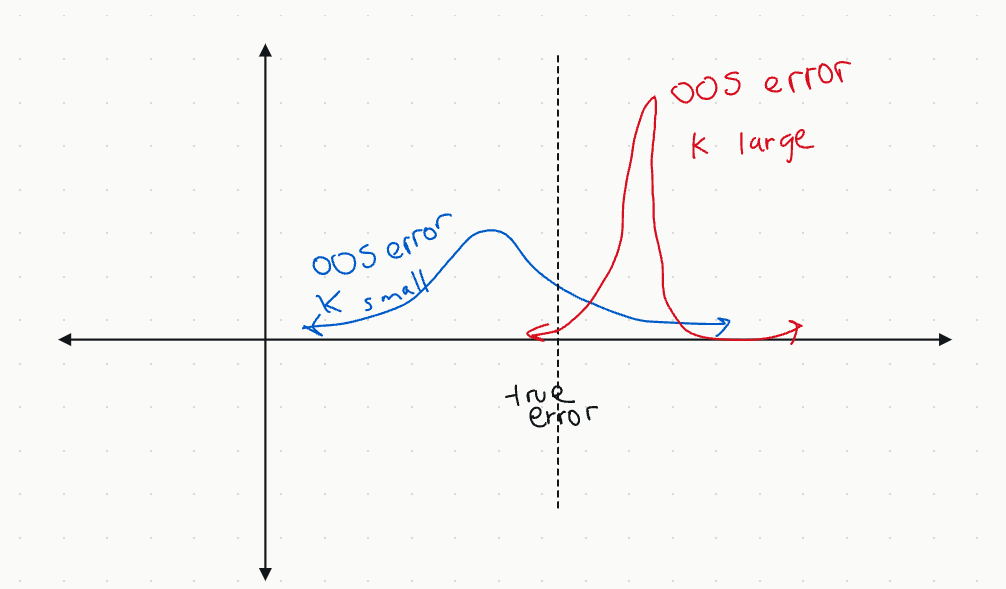
\includegraphics[width=0.6\textwidth]{oos-error-varying-by-K}
			\caption{Visualizing how the proportion of $\mathbb{D}$ we use for
			$\mathbb{D}_{\text{test}}$ affects the stability of out-of-sample error
			metrics.}
			\label{fig:oos-error-vary-by-K}
		\end{figure}
		\item \textit{How do we perform the split?} By default, we do it at \text{random}.
		If $\mathbb{D}$ happened to come with time dependence, like a time series
		(not the subject of this class), then we could use that inherent order. An example
		is the stock market prices, or sports statistics. However, for this class,
		the split will in general be made randomly.
	\end{enumerate}
	\section*{Incorporating Out-of-Sample Metrics in Modeling}
	\begin{figure}
		\centering
		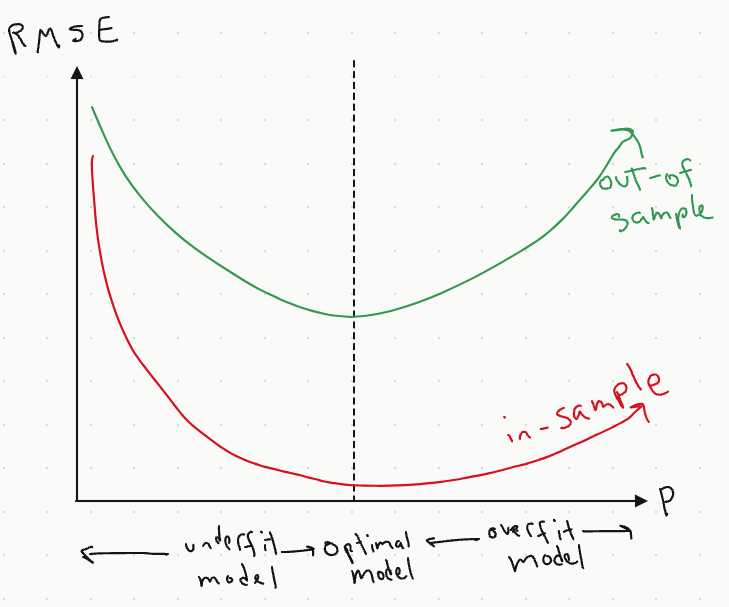
\includegraphics[width=0.6\textwidth]{p-vs-RMSE-oos-insample}
		\caption{Plot of how in-sample and out-of-sample RMSE change
		as $p$ increases.}
		\label{fig:oos-insamp-rmse-p}
	\end{figure}
	Figure~\ref{fig:oos-insamp-rmse-p} plots $p$, the number of predictors
	used, against the $RMSE$ for both out-of-sample metrics and in-sample
	metrics. We see that out-of-sample $RMSE$ tends to be large
	even as in-sample drops close to $0$, since it can better
	detect that we add junk features. The optimal model is shown,
	which corresponds to where the out-of-sample RMSE is lowest.
	
	Figure~\ref{fig:measure-build-test-predict} extends the picture we
	drew in lecture 2, incorporating into the modeling framework our new
	ideas about $\mathbb{D}_{\text{train}}$ and $\mathbb{D}_{\text{test}}$.
	Computing the out-of-sample predictions on $\mathbb{D}_{\text{test}}$
	provides us with honest validation.
	\begin{figure}
		\centering
		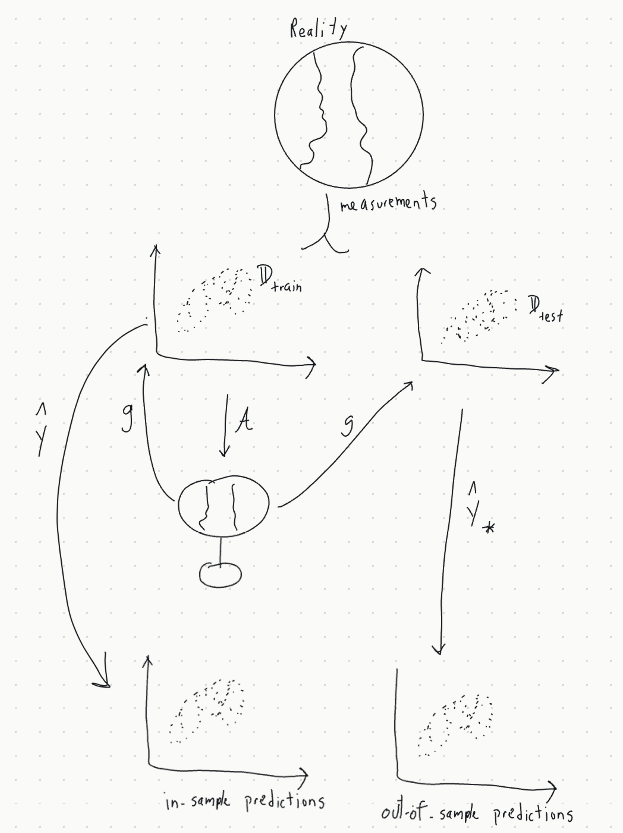
\includegraphics[width=0.6\textwidth]{measure-build-test-predict-process}
		\caption{The framework of measuring a response from a phenomenon,
		building a model $g$ on $\mathbb{D}_{\text{train}}$, then gauging the
		performance of $g$ by applying $g$ on $\mathbb{D}_{\text{train}}$
		to compute in-sample metrics and applying $g$ on $\mathbb{D}_{\text{test}}$
		to compute out-of-sample metrics.}
		\label{fig:measure-build-test-predict}
	\end{figure}
	
	Figure~\ref{fig:measure-build-test-predict-v2} shows an alternative view of
	the same process depicted in Figure~\ref{fig:measure-build-test-predict}.
	\begin{figure}
		\centering
		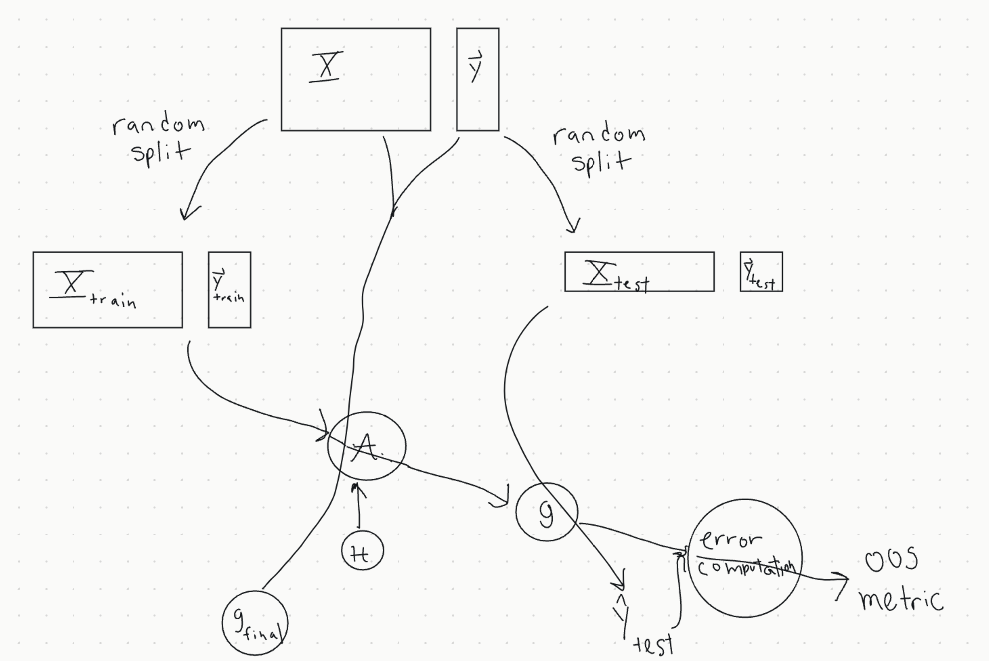
\includegraphics[width=0.8\textwidth]{measure-build-test-predict-process-v2}
		\caption{Alternative view of the process depicted in Figure~\ref{fig:measure-build-test-predict}.}
		\label{fig:measure-build-test-predict-v2}
	\end{figure}
	Keep in mind that if, say, we apply OLS with 2 features and 1000 rows,
	then in-sample will be close to out-of-sample, since $p$ is much smaller
	than $n$ and we are likely not doing any ``funny business".
	
	Note that we could use $g$ that we obtain from working with $\mathbb{D}_{\text{train}}$
	to predict, but since we did not use all of the data, we unnecessarily incur estimation
	error. Instead, we use $g_{\text{final}}$ which is built by applying
	the algorithm on the full $\mathbb{D}$. Why should $g_{\text{final}}$ be okay
	to use given we got $g$ and our out-of-sample metrics from our algorithm and $g$?s
	Because the out-of-sample metrics computed using $g$ are conservative with respect to
	$g_{\text{final}}$, assuming stationary phenomenon.
	
	As we can see, a main (and very important) reason we partition $\mathbb{D}$
	into $\mathbb{D}_{\text{train}}$ and $\mathbb{D}_{\text{test}}$ is to get a sense
	of $g_{\text{final}}$ will do when we build it with \textit{all the data}
	(with $\mathbb{D}$).
	\section*{$K$-Fold Cross-Validation}
	When we split $\mathbb{D}$ into a $\mathbb{D}_{\text{train}}$ and $\mathbb{D}_{\text{test}}$
	with $K:=\frac{n}{n_{\text{test}}}$, we need to keep in mind that if $K$ is large,
	the out-of-sample metrics will be stable. We can apply the following procedure:
	\begin{enumerate}[label=(\alph*)]
		\item \textbf{Step 0}: Start with your data set $\mathbb{D}$:
		\begin{align*}
			\begin{bmatrix}
				{} & {} & {}\\
				{} & X & {}\\
				{} &   & {}
			\end{bmatrix}
			\begin{bmatrix}
				{}\\
				\mathbf{y}\\
				{}
			\end{bmatrix}
		\end{align*}
		\item \textbf{Step 1}: Perform 1 split, where we let the first
		$n_{\text{test}}$ rows (observations) be $\mathbb{D}_{\text{test}}$, while the
		rest are $\mathbb{D}_{\text{train}}$:
		\begin{align*}
			\begin{bmatrix}
				{} & X_{\text{test\ \  }} & {}
			\end{bmatrix}
			&
			\begin{bmatrix}
				\mathbf{y}_{\text{test\ \ }}
			\end{bmatrix}\\
			\begin{bmatrix}
				{} & {} & {}\\
				{} & X_{\text{train}} & {}
			\end{bmatrix}
			&
			\begin{bmatrix}
				{}\\
				\mathbf{y}_{\text{train}}
			\end{bmatrix}
		\end{align*}
		From this step we get out-of-sample residual (error) vector $\mathbf{e}_{*1}$
		of length $K$.
		\item \textbf{Step 2}: Next we split by taking the \textit{second} $n_{\text{test}}$
		rows for $\mathbb{D}_{\text{test}}$, while using the remaining for $\mathbb{D}_{\text{train}}$:
		\begin{align*}
			\begin{bmatrix}
				{} & X_{\text{train}} & {}
			\end{bmatrix}
			&
			\begin{bmatrix}
				\mathbf{y}_{\text{train}}
			\end{bmatrix}\\
			\begin{bmatrix}
				{} & X_{\text{test\ \ }} & {}
			\end{bmatrix}
			&
			\begin{bmatrix}
				\mathbf{y}_{\text{test\ \ }}
			\end{bmatrix}\\
			\begin{bmatrix}
				{} & X_{\text{train}} & {}
			\end{bmatrix}
			&
			\begin{bmatrix}
				\mathbf{y}_{\text{train}}
			\end{bmatrix}
		\end{align*}
		Then we get another out-of-sample residual (error) vector $\mathbf{e_{*2}}$
		of length $K$. Notice that though it appears we have multiple training sets, that's
		not the case. The point being emphasized is that the second portion of the
		overall $\mathbb{D}$ (and hence $X$ and $\mathbf{y}$) is being used for testing,
		and the remaining for training.
		\item \textbf{Step $K$}: We continue until we perform the $K$th split, similar to before,
		and a corresponding residual vector $\mathbf{e}_{*K}$.
	\end{enumerate}
	At the end, we have a vector $\mathbf{e}_*$ of length $n$ obtained by concatenating the
	$K$ vectors each of length about $n_{\text{test}} = n/K$:
	\begin{align*}
		\mathbf{e}_* = \begin{bmatrix}
			\mathbf{e}_{*1}\\
			\mathbf{e}_{*2}\\
			\vdots\\
			\mathbf{e}_{*K}
		\end{bmatrix}
	\end{align*}
	Each split ``crosses $\mathbf{D}_{\text{test}}$" ``over", hence the procedure is
	named \textbf{cross-validation}, or \textbf{$K$-fold CV}. This implies stability
	in the OOS metrics.
	
	From the $K$ residual error vectors $\mathbf{e}_{*1},\mathbf{e}_{*2},\ldots,\mathbf{e}_{*K}$,
	we have corresponding out-of-sample metrics:
	\begin{align*}
		oosRMSE_1,oosRMSE_2,\ldots,oosRMSE_K
	\end{align*}
	Then we can define a standard deviation:
	\begin{align*}
		S_{oosRMSE}:=\sqrt{\frac{1}{K-1}\sum_{\ell=1}^{K}
			\left(oosRMSE_{\ell} - \overline{oosRMSE}\right)^2}
	\end{align*}
	and now we have a confidence interval real standard deviation $\sigma_{oosRMSE}$
	of the error:
	\begin{align*}
		CI_{\sigma, 95\%}=\left[
		\overline{oosRMSE} \pm 2\frac{S_{oosRMSE}}{\sqrt{K}}
		\right]
	\end{align*}
	This gives an approximate on the range of how sure we can be of future performance.
	\pagebreak
	\printbibliography
\end{document}